\documentclass[11pt]{article}

\usepackage[utf8]{inputenc}
\usepackage[portuges]{babel}
\usepackage{indentfirst}
\usepackage{natbib}
\usepackage{graphicx}
\usepackage{adjustbox}
\usepackage{geometry}
 \geometry{
    a4paper,
    total={130mm,227mm},
    left=40mm,
    right=40mm,
    top=30mm,
    bottom=30mm
}
\setlength\abovecaptionskip{-2pt}
 
\renewcommand{\contentsname}{Índice}

\begin{document}

\begin{titlepage}
    \begin{center}
        
\includegraphics[width=0.3\textwidth]{images/capa/EscolaEngenhariaUM.jpeg}
    
        \vspace{1cm}
        
        \textbf{\LARGE Comunicações por Computador}
    
        \vspace{0.5cm}
        \textbf{\Large Trabalho Prático 1}

        \vspace{1.3cm}
        
        \textbf{\large Luís Pedro Oliveira de Castro Vieira A89601 \\
        José Pedro de Castro Ferreira A89572 \\
        Luís Enes Sousa A89597}

        \vspace{1.5cm}
        \begin{figure}[hbt!]
            \minipage{0.32\textwidth}
                \frame{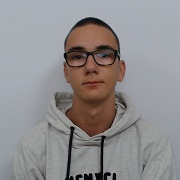
\includegraphics[width=\linewidth]{images/capa/massini.jpg}}
                \centering
                \captionsetup{A89601}
            \endminipage\hfill
            \minipage{0.32\textwidth}
                \frame{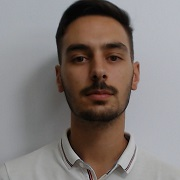
\includegraphics[width=\linewidth]{images/capa/8free.jpg}}
                \centering
                \captionsetup{A89572}
            \endminipage\hfill
            \minipage{0.32\textwidth}
                \frame{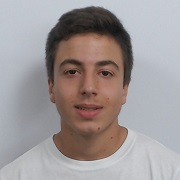
\includegraphics[width=\linewidth]{images/capa/80.jpeg}}
                \centering
                \captionsetup{A89597}
            \endminipage
        \end{figure}
    \end{center}
\end{titlepage}

\tableofcontents
\thispagestyle{empty}
\cleardoublepage

\setcounter{page}{1}


%-----------------------------------------------------------------%
\section{Protocolos da Camada de Transporte}
\vspace{0.5cm}


%-----------------------------------------------------------------%
\subsection{Pergunta 1}

\textbf{Inclua no relatório uma tabela em que identifique, para cada comando executado, qual o protocolo de aplicação, o protocolo de transporte, porta de atendimento e overhead de transporte, como ilustrado no exemplo seguinte:}

\begin{table}[hbt!]
    \begin{adjustbox}{width=\textwidth}
        \begin{tabular}{|c|c|c|c|c|}
\hline
& Protocolo de Aplicação & Protocolo de Transporte & Porta de Atendimento & Overhead de Transporte \\
\hline
Ping         & PING        &  -    &   -     &   -   \\
\hline
traceroute   & TRACEROUTE  & UDP   & 33434   & 8     \\
\hline
telnet       & TELNET      & TCP   & 23      & 40    \\
\hline
ftp          & FTP         & TCP   & 21      & 20    \\
\hline
Tftp         & TFTP        & UDP   & 69      & 8     \\
\hline
browser/http & HTTP        & TCP   & 80      & 20    \\
\hline
nslookup     & DNS         & UDP   & 53      & 8     \\
\hline
ssh          & SSH         & TCP   & 22      & 40    \\
\hline
        \end{tabular}
    \end{adjustbox}
\end{table}

O comando  \textit{ping} não tem um protocolo de transporte correspondente, pois este executa no nível 3 da camada protocolar (Network Layer).

Para preencher a coluna do protocolo de transporte, verificamos qual era o protocolo de nível 4 associado à trama correspondente.

Em relação à coluna da porta de atendimento, esta foi preenchida analisando a porta de destino da trama enviada pelo host.

Quanto à coluna do overhead de transporte, foi preenchida de duas maneiras diferentes: uma para as tramas UDP e outra para as TCP. Como se pode ver na figura 2, o overhead duma trama UDP é calculado pela diferença entre  \textit{Total length} e  \textit{Data length} (40 - 32 = 8 bytes). Isto acontece em todas as tramas do protocolo UDP, logo o overhead de transporte de tramas UDP é sempre 8 bytes. Quanto às tramas TCP, o overhead de transporte está especificado no header.

\vspace{0.5cm}

\begin{figure}[hbt!]
    \centering
    \frame{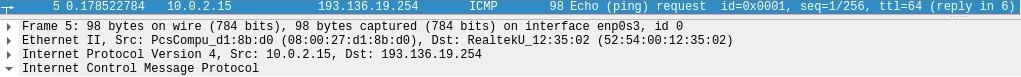
\includegraphics[width=\textwidth]{images/Q1/ping.png}}
    \caption{Trama ping}
\end{figure}

\begin{figure}[hbt!]
    \centering
    \frame{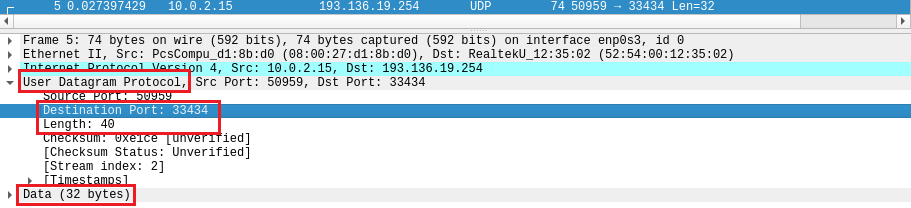
\includegraphics[width=\textwidth]{images/Q1/traceroute.png}}
    \caption{Trama traceroute}
\end{figure}

\begin{figure}[hbt!]
    \centering
    \frame{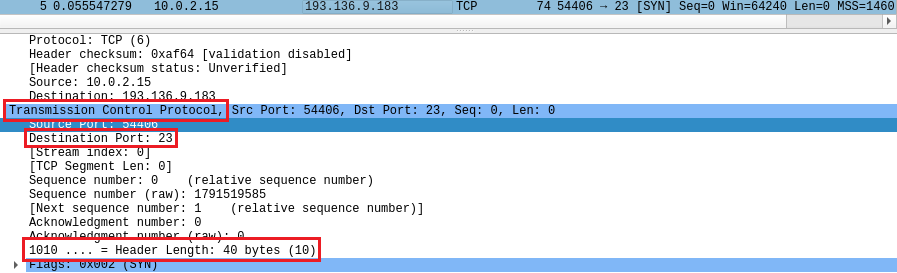
\includegraphics[width=\textwidth]{images/Q1/telnet.png}}
    \caption{Trama telnet}
\end{figure}

\begin{figure}[hbt!]
    \centering
    \frame{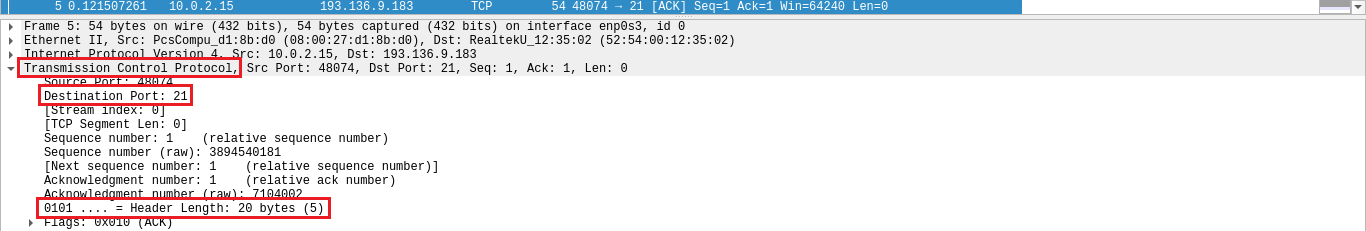
\includegraphics[width=\textwidth]{images/Q1/ftp.PNG}}
    \caption{Trama ftp}
\end{figure}

\begin{figure}[hbt!]
    \centering
    \frame{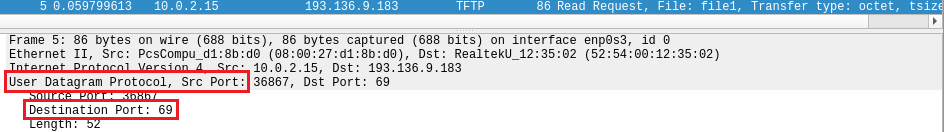
\includegraphics[width=\textwidth]{images/Q1/tftp.PNG}}
    \caption{Trama Tftp}
\end{figure}

\begin{figure}[hbt!]
    \centering
    \frame{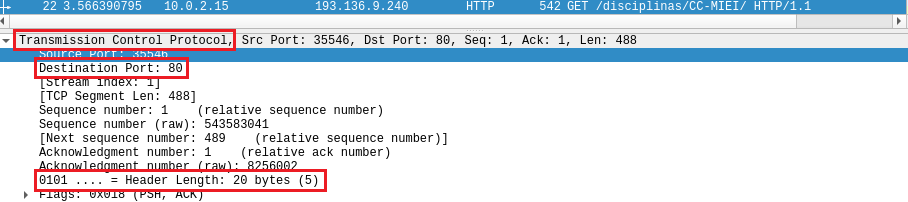
\includegraphics[width=\textwidth]{images/Q1/browser.PNG}}
    \caption{Trama browser/http}
\end{figure}

\begin{figure}[hbt!]
    \centering
    \frame{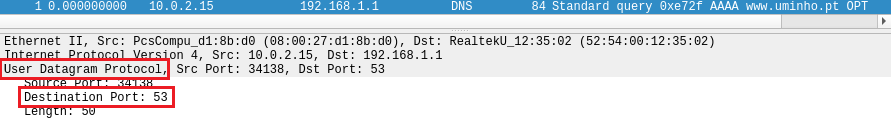
\includegraphics[width=\textwidth]{images/Q1/nslookup.PNG}}
    \caption{Trama nslookup}
\end{figure}

\begin{figure}[hbt!]
    \centering
    \frame{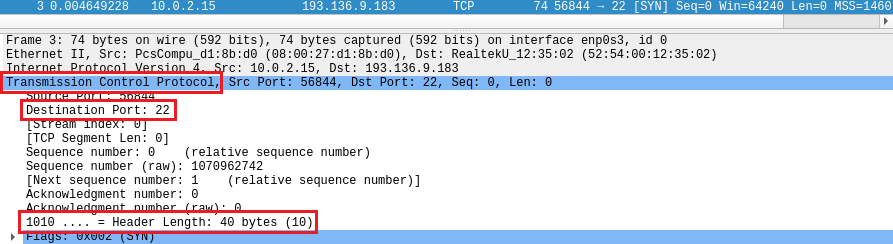
\includegraphics[width=\textwidth]{images/Q1/ssh.PNG}}
    \caption{Trama ssh}
\end{figure}


%-----------------------------------------------------------------%
\clearpage
\subsection{Pergunta 2}

\textbf{Uma representação num diagrama temporal das transferências da file1 por FTP e TFTP respetivamente. Se for caso disso, identifique as fases de estabelecimento de conexão, transferência de dados e fim de conexão. Identifica também claramente os tipos de segmentos trocados e os números de sequência usados quer nos dados como nas confirmações.}

\subsubsection{FTP}

O protocolo FTP, \textit{File Transfer Protocol}, pode ser executado em dois modos: passivo e ativo, dependendo de quem começa a conexão entre o cliente e o servidor.

\vspace{0.5cm}

\par \textbf{-$>$ FTP Ativo}

\vspace{0.25cm}

Se a conexão for inicializada por parte do servidor, esta será ativa, ou seja, tanto o servidor como o cliente necessitarão de disponibilizar e abrir portas para o tráfego circular.

\vspace{0.5cm}

\par \textbf{-$>$ FTP Passivo}

\vspace{0.25cm}

Por outro lado, se a conexão for inicializada por parte do cliente, esta será passiva, isto é, é indispensável que o servidor abra portas de forma a receber tráfego, mas o mesmo não é necessário para o cliente.

\begin{figure}[hbt!]
    \centering
    \frame{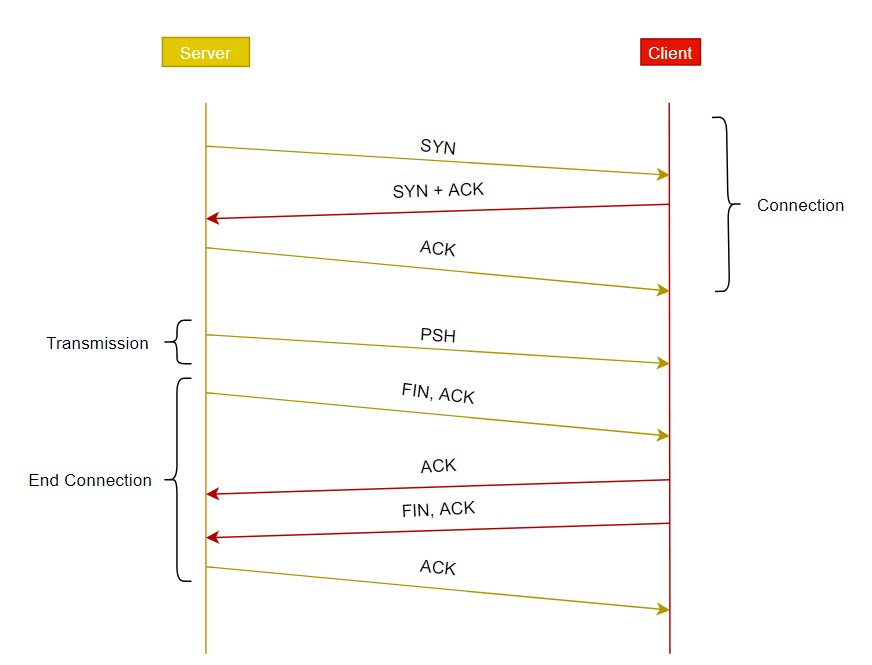
\includegraphics[width=0.6\textwidth]{images/Q2/FTPdiag.jpg}}
    \caption{Diagrama Temporal de uma Conexão FTP}
\end{figure}

O protocolo FTP faz uso de um par de conexões entre o cliente e o servidor, sendo que a primeira conexão a ser estabelecida é com a porta 20 do servidor e a segunda com a porta 21.

Os servidores, ao abrirem a porta 21, começam à escuta por conexões de entrada do cliente, os quais se ligam a esta para iniciar as operações de transferência de ficheiros. No entanto, e algo importante a notar, é a necessidade extrema e estrita da porta 20, a qual possibilita efetivamente estas operações.

\clearpage
Ao analisarmos a figura 1 afirmamos, com certezas, que a conexão se inicia com o servidor a enviar um segmento SYN, indicando que os números de sequência se devem sincronizar de forma a iniciar a conexão. De seguida, o cliente responde com um segmento SYN e uma trama ACK, o qual permite inferir que houve sucesso na receção do segmento SYN previamente enviado pelo servidor.

Da mesma forma que o cliente respondeu ao servidor a afirmar que recebeu com sucesso o segmento SYN, este último efetua o mesmo procedimento enviando uma trama ACK ao cliente.

Desta forma, e estando estabelecida a conexão, o servidor envia para o cliente os dados que são pretendidos, iniciando-se a fase de transmissão.

Posteriormente, e de forma a finalizar a conexão, inicia-se uma nova troca de segmentos e tramas entre o cliente e o servidor. Neste caso, o servidor começa por enviar um segmento FIN ao cliente a informar que terminou a transmissão de dados, ao qual o cliente responde, tal como na fase da conexão, com um segmento FIN e uma trama ACK a informar que recebeu com sucesso o segmento anterior. Por fim, o servidor envia uma trama ACK a confirmar o sucesso na receção do segmento FIN anterior, finalizando, assim, a conexão entre ambos.

\subsubsection{TFTP}

\begin{figure}[hbt!]
    \centering
    \frame{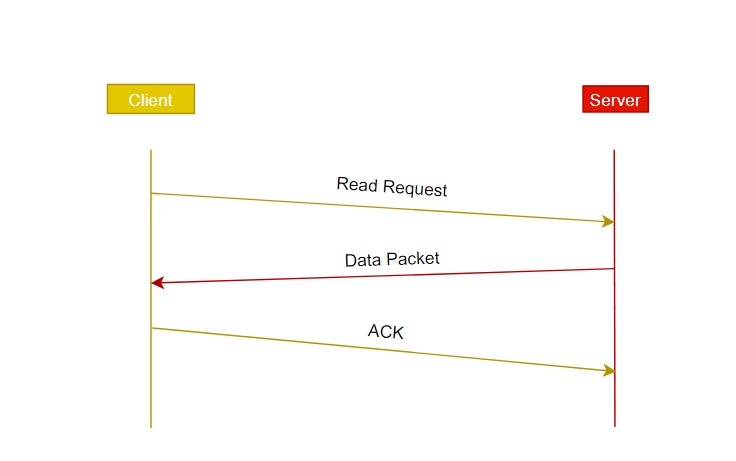
\includegraphics[width=0.6\textwidth]{images/Q2/TFTPdiag.jpg}}
    \caption{Diagrama Temporal de uma Conexão TFTP}
\end{figure}

Como podemos confirmar pela figura acima, o cliente começa por enviar um  \textit{Read Request} ao servidor, que, posteriormente, irá enviar um pacote de dados e, por fim, o cliente responde com uma trama ACK a informar o sucesso da receção desses dados.

Neste protocolo, todas as transferências começam com um pedido de leitura ou com um pedido de escrita de um ficheiro e, ao mesmo tempo, uma requisição de conexão por parte do cliente. Se o servidor atender ao pedido, a conexão é estabelecida e o ficheiro é enviado em blocos de comprimento fixo. Caso o comprimento do pacote seja superior ao limite, dá-se fragmentação do pacote e são enviados em vários pacotes, com o mesmo comprimento.


%-----------------------------------------------------------------%
\clearpage
\subsection{Pergunta 3}

\textbf{Com base nas experiências realizadas, distinga e compare sucintamente as quatro aplicações de transferência de ficheiros que usou nos seguintes pontos (i) uso da camada de transporte; (ii) eficiência na transferência; (iii) complexidade; (iv) segurança;}

\subsubsection{Uso da camada de transporte}
\begin{enumerate}
  \item \textbf{SFTP}:\\
  Usufrui do protocolo TCP
  \item \textbf{FTP}:\\
  Usufrui do protocolo TCP
  \item \textbf{TFTP}:\\
  Usufrui do protocolo UDP
  \item \textbf{HTTP}:\\
  Usufrui do protocolo TCP
\end{enumerate}

\subsubsection{Eficiência na transferência}
\begin{enumerate}
  \item \textbf{SFTP}:\\
  Similar ao protocolo FTP, mas utiliza dados encriptados usufruindo do SSH para tal efeito.
  \item \textbf{FTP}:\\
  Como vimos previamente na questão 2, o protocolo FTP garante, por usufruir do protocolo TCP e através da troca de \textbf{ACK}nowledgments, que os segmentos serão efetivamente transmitidos. Isto, porém, peca na eficência uma vez que é necessário esperar pelo ACK para poder continuar. Comparativamente ao SFTP, por não fazer uso da encriptação, torna possível a interceção dos segmentos por parte de terceiros.
  \item \textbf{TFTP}:\\
  Desde início, por usufruir do protocolo UDP, torna-se menos viável, pois não utiliza ACKs para confirmar a receção bem sucedida dos pacotes. Como não garante a entrega dos mesmos, é necessário que haja a retransmissão destes em caso de falha. No entanto, quando bem sucedido, é mais rápido que o protocolo FTP.
  \item \textbf{HTTP}:\\
  Este protocolo permite que, numa só ligação TCP, sejam enviados múltiplos HTTP requests
  sem ser necessário esperar pelas respetivas respostas.
\end{enumerate}

\subsubsection{Complexidade}
\begin{enumerate}
  \item \textbf{SFTP}:\\
  Por ser um protocolo bastante fiável, que permite acesso, transferência e gestão de dados, o SFTP acaba por ser também deveras complexo, pois todas estas funcionalidades possuem elevados custos de processamento.
  \item \textbf{FTP}:\\
  É capaz de suportar diferentes pedidos para transferência de dados em paralelo, no qual cada uma das transferências inicializa uma nova conexão, fazendo com que existam diferentes velocidades de transferência. Devido a este efeito de criação regular de novas conexões, o protocolo FTP releva-se, também, bastante complexo.
  \item \textbf{TFTP}:\\
  O protocolo TFTP é, tal como o nome indica, \textit{Trivial}, ou seja, uma alternativa simplificada do protocolo FTP. Por consequente, o TFTP suporta um menor número de funcionalidades, o que, juntamente com o facto de se basear no protocolo UDP para transporte, acaba por afetar a complexidade deste protocolo em geral. Podemos, então, concluir que o TFTP não se trata de um protocolo complexo.
  \item \textbf{HTTP}:\\
  Este último protocolo é capaz de garantir confiança, escalabilidade e desacoplamento de sistemas e, para além disso, oferece um suporte para hipermedia para redes complexas ou redes diferentes e não confiáveis. Por isto, o protocolo HTTP acaba por se tornar complexo.
\end{enumerate}

\subsubsection{Segurança}
\begin{enumerate}
  \item \textbf{SFTP}:\\
  Como mencionado previamente, o protocolo SFTP faz uso do SSH (\textit{Secure Shell}) permitindo-nos, então, concluir que se trata de um protocolo efetivamente seguro. No entanto, é necessário entender que o SSH faz uso de uma arquitetura em camadas, nomeadamente de uma camada de transporte, uma de autenticação e uma de conexão. No que toca ao assunto abordado, a segurança, ao nível do transporte existe um auxílio por parte do protocolo TCP/IP e fornece encriptação, autenticação do servidor e proteção na íntegra dos dados. Já ao nível da camada de autenticação, esta é responsável por manipular a autenticação dos clientes.
  \item \textbf{FTP}:\\
  Por não fornecer encriptação de dados, o protocolo FTP tornou-se conhecido pelas suas diversas falhas na segurança. Como as transmissões não se encontram encriptadas, permite que qualquer pessoa seja capaz de efetuar uma captura de pacotes na rede, tendo acesso a diversas informações particulares, como nomes de utilizadores, palavras-passe, etc. Isto acaba por demonstrar que o protocolo é realmente muito pouco seguro.
  \item \textbf{TFTP}:\\
  Na utilização do protocolo TFTP não é necessário uma autenticação, o que torna, de imediato, evidente que este procotolo não é o mais seguro, visto não proteger os dados que estão a ser transferidos.
\clearpage
  \item \textbf{HTTP}:\\
  Na utilização do protocolo HTTP, toda a informação é representada em texto e não se encontra encriptada, logo, os dados poderão ser adulterados muito facilmente, o que o torna muito inseguro.
\end{enumerate}


%-----------------------------------------------------------------%
\vspace{0.5cm}
\subsection{Pergunta 4}

\textbf{As características das ligações de rede têm uma enorme influência nos níveis de Transporte e de Aplicação. Discuta, relacionando a resposta com as experiências realizadas, as influências das situações de perda ou duplicação de pacotes IP no desempenho global de Aplicações fiáveis (se possível, relacionando com alguns dos mecanismos de transporte envolvidos).}

\vspace{0.5cm}

A perda e duplicação de pacotes IP nos níveis de Transporte e de Aplicação são bastante comuns, tornando-se, cada vez mais, um desafio combater estas situações. Um exemplo desta situação é a LAN3, que se encontra na topologia de rede fornecida junto com o enunciado. Os protocolos de transporte estudados, \textbf{TCP} e \textbf{UDP}, procuram tentar resolver estes problemas.
Como já referimos, o protocolo TCP deteta e corrige erros, pelo que, quando são encontrados pacotes com erros, ocorre uma tentativa de retransmissão do mesmo. No entanto, com esta retransmissão, acontece também uma redução no débito de transmissão e, consequentemente, as filas dos routers vão sendo esvaziadas. Posteriormente, o débito de transmissão é aumentado, sendo este um aumento global.
Por outro lado, o protocolo UDP, apesar de detetar erros, não os corrige: os pacotes com erros são simplesmente descartados, uma vez que este protocolo não possui nenhum campo que tenha como função a correção de erros. Sendo assim, não é possível detetar perdas de pacotes. A questão de como resolver este problema é respondida com a dependência de um protocolo que se encontra acima do protocolo UDP, cuja função é identificar pacotes pelo seu ID ou número de sequência, conseguindo, deste modo, saber se todos os pacotes foram recebidos, ou até se algum se perdeu no processo.

\begin{figure}[hbt!]
    \centering
    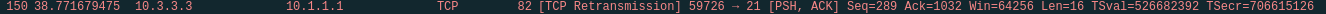
\includegraphics[width=1\textwidth]{images/Q4/erroftp.PNG}
    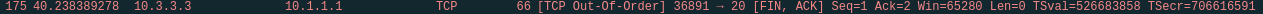
\includegraphics[width=1\textwidth]{images/Q4/erroftp2.PNG}
    \caption{Computador a fazer download usando o FTP}
    \label{fig:my_label}
\end{figure}

\begin{figure}[hbt!]
    \centering
    
\includegraphics[width=1\textwidth]{images/Q4/tftp erro.PNG}
    \caption{Computador a fazer download usando o TFTP}
    \label{fig:my_label}
\end{figure}

As figuras 11 e 12 mostram o download do ficheiro \textit{file1.txt}, usando FTP e TFTP. Durante a captura, em ambas as situações, a maior parte dos envios foram bem sucedidos. No entanto, após várias tentativas, podemos apurar que, por vezes, eram encontrados erros. 
Quando usado o FTP (como podemos ver pela Figura 11) existiam segmentos ACK que acabavam repetidos, mas, mesmo assim, o ficheiro acabava por conseguir chegar ao seu destino final. Ao usar o TFTP, o ficheiro não chegava ao seu destino final e o host acabava por perder muito tempo até se aperceber que tal tinha acontecido. No entanto, nos casos em que as transferências era feitas com sucesso, a transferência usando TFTP era mais rápida do que se fosse feita com o FTP.

Assim, podemos concluir que, caso o ficheiro a transferir seja pequeno ou a velocidade seja a prioridade, o TFTP deverá ser a aplicação a utilizar. Caso a prioridade seja garantir que o ficheiro chega ao destino (grandes quantidades de dados) devemos usar o FTP, uma vez que assegura a transferência de todos os dados, ainda que seja um pouco mais demorado.


%-----------------------------------------------------------------%
\clearpage
\section{Conclusão}

Terminada a realização deste trabalho prático, conseguimos aprofundar e ver em prática os nossos conhecimentos acerca dos diversos Protocolos da Camada de Transporte. Para além destes, foram ainda objetos de estudo múltiplos Protocolos da Camada de Aplicação. Entre os temas explorados encontram-se os seus comportamentos, assim como as vantagens e desvantagens da utilização dos mesmos.
Com o intuito de consolidar estes conhecimentos, e com o auxílio da ferramenta \textit{Core} e \textit{Wireshark}, foram realizadas algumas demonstrações, possibilitando a visualização de variados procedimentos e processos de transferência de dados, em diferentes protocolos.

Posto isto, podemos conlcuir que, se quisermos realizar uma transferência de dados e garantir que todos os dados enviados são recebidos, temos de escolher uma aplicação que utilize o protocolo TCP, apesar deste não ser o protocolo mais eficiente, uma vez que deteta e corrige erros. Por outro lado, se a perda de pacotes não for um problema maior, devemos optar pelo protocolo UDP, aproveitando, deste modo, a velocidade máxima de transferência possível.

Assim, terminamos este trabalho prático afirmando entender melhor os temas abordados e descritos durante a realização do mesmo.
\end{document}
